% Packages {{{
\documentclass[lettersize,journal]{IEEEtran}
\usepackage{algorithmic}
\usepackage{algorithm}
\usepackage{amsmath,amsfonts}
\usepackage{array}
\usepackage{arydshln} % for horizontal dashed lines in table
\usepackage{balance}
\usepackage{cite}
\usepackage{gensymb} % for degrees symbol
\usepackage{graphicx}
\usepackage{stfloats}
\usepackage[caption=false,font=normalsize,labelfont=sf,textfont=sf]{subfig}
\usepackage{tabularx}
\usepackage{textcomp}
\usepackage{tikz}
\usetikzlibrary{calc}
\usetikzlibrary{math}
\usepackage{url}
\usepackage{verbatim}
\usepackage{xcolor}
%}}}
% Setup {{{
\hyphenation{op-tical net-works semi-conduc-tor IEEE-Xplore}
\title{MEng in Electronic \& Computer Engineering}
\author{Andrew Whelan, \emph{Dublin City University},
   Prof. Conor Brennan, \emph{Dublin City University}}
% The paper headers
\markboth{MEng in Electronic \& Computer Engineering}%
{Shell \MakeLowercase{\textit{et al.}}:
   Modelling of Diffuse Scattering Effects for Outdoor Ray Tracing}
% Title {{{
\begin{document}
\maketitle
%}}}
%}}}
% Abstract {{{
\begin{abstract}
   A heuristic model of diffuse scattering is elaborated and applied to a setup
   consisting of a plane wave incident on a sinusoidally shaped wall.
   Results are compared to full-wave method-of-moments (MoM) model, and also to
   Geometrical Optics (GO) and Physical Optics (PO) approximations.
\end{abstract}
%}}}
% IEEE Keywords {{{
\begin{IEEEkeywords}
   Diffuse Scattering, Diffuse Reflection, Channel Model, Ray Tracing, Ray Shooting.
\end{IEEEkeywords}
%}}}
% Introduction {{{
\section{Introduction}
   \IEEEPARstart{T}{his} is the intro.
%}}}
% Models {{{
\section{Models}
% Effective Roughness Model {{{
\subsection{Effective Roughness Model}
% Pre Fig.1 {{{
        This model is a modification of Geometrical Optics in which, in addition to the
        specular component, each point impinging on the middle of a surface element $dW$
        gives a diffuse contribution $dE_d$ to the scattered field $E_s$ whose amplitude
        $\left| dE_d \right|$ is given by
        \begin{equation} \label{eq:scatteringAmpER}
           \left| dE_d \right| \propto \sqrt{\frac{dW \cos \theta_i \cos \theta_d}{\pi}}
           \frac{1}{r_i r_d}
        \end{equation}
        with the constant of proportionality depending on the incident amplitude and a
        scattering parameter $S$. Specifically, we have
        \begin{subequations}
            \begin{align}
                \left| dE_d \right| &= S \Upsilon \sqrt{dW}, \quad \text{where} \\
                \Upsilon &= \sqrt{\frac{60 G_t P_t \cos \theta_i \cos \theta_d}{\pi}}
                \frac{1}{r_i r_d}
            \end{align}
        \end{subequations}
        \subsubsection{Uniform Plane Wave Incident on PEC}    
            We start with a setup as per Figure~\ref{fig:planeWavePEC}. 
            \begin{subequations}
                \begin{align}
                    k_i &= \sin (\theta_i) \text{e}_x - \cos (\theta_i) \text{e}_y \\
                    k_r &= \sin (\theta_i) \text{e}_x + \cos (\theta_i) \text{e}_y \\
                    k_d &= \sin (\theta_d) \text{e}_x + \cos (\theta_d) \text{e}_y
                \end{align}
            \end{subequations}
%}}}
            % Fig.1 {{{
            \begin{figure}[H] 
            \begin{center}
            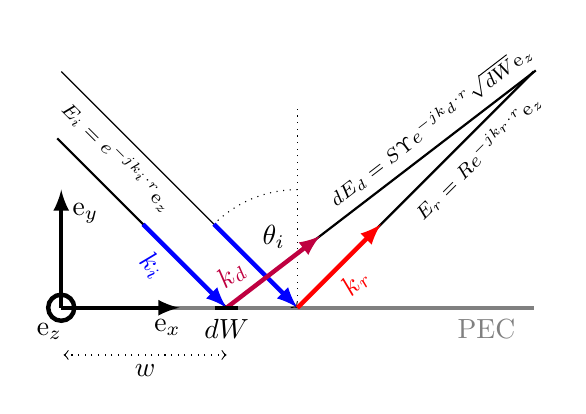
\begin{tikzpicture}[scale=1.5]
            \newcommand{\drawLabelledArrow}[9]{%
                \tikzmath{
                    \xArrowStart = #1; 
                    \yArrowStart = #2;
                    \arrowLen = #3; 
                    \arrowAngle = #4;
                    \labelAngleShift = #7;
                    \xArrowEnd = \xArrowStart + \arrowLen * cos(\arrowAngle);
                    \yArrowEnd = \yArrowStart + \arrowLen * sin(\arrowAngle);
                }
                % Define the text and color as regular TeX macros
                \def\arrowLabel{#5}%
                \def\arrowColor{#6}%
                \def\arrowStyle{#8}
                \def\labelStyle{#9}
                % Draw
                \draw[#8, \arrowColor] 
                    (\xArrowStart, \yArrowStart) -- (\xArrowEnd, \yArrowEnd)
                    node[#9, rotate=\arrowAngle+\labelAngleShift]
                        {\arrowLabel};
            }
            % Call the macro with: xStart, yStart, length, angle, label, label offset,
%             color
            % Wall
            \tikzmath{
                    \xObstacleStart = 0;            
                    \yObstacleStart = 0;            
                    \obstacleLen = 4;               
                    \obstacleAngle = 0;            
                    \xObstacleCentre = 0.5*\obstacleLen*cos(\obstacleAngle);
                    \yObstacleCentre = 0.5*\obstacleLen*sin(\obstacleAngle);
            }
            \def\obstacleLabel{PEC}
            \def\obstacleColor{gray}
            \def\obstacleArrowStyle{ultra thick}
            \drawLabelledArrow{\xObstacleStart}{\yObstacleStart}{\obstacleLen}
                {\obstacleAngle}{\obstacleLabel}{\obstacleColor}{0}{\obstacleArrowStyle}
                {pos=0.9,below}
            % Incident Ray
            \tikzmath{
                    \xIncidentStart = \xObstacleStart + \xObstacleCentre);
                    \yIncidentStart = \yObstacleStart + \yObstacleCentre);
                    \incidentAngle = \obstacleAngle + 135;
                    \incidentLen =
                        \obstacleLen/(abs(2*cos(\incidentAngle)));%\obstacleLen * ; 
            }
            \def\incidentLabel{\begingroup \scriptsize $E_i = e^{-jk_i \cdot r}
                \text{e}_z$ \endgroup}%= E_0 e^{-jk_i \cdot r} \text{e}_z$}
            \def\incidentColor{black}
            \def\incidentArrowStyle{<-}
            \drawLabelledArrow{\xIncidentStart}{\yIncidentStart}{\incidentLen}
                {\incidentAngle}{\incidentLabel}{\incidentColor}{180}
                {\incidentArrowStyle}{pos=0.7,below}
            % Normal Ray
            \tikzmath{
                    \normalLen = \obstacleLen*(0.4); 
                    \xNormalStart = (\normalLen/2)*sin(\obstacleAngle) + \xObstacleStart +
                        \xObstacleCentre;
                    \yNormalStart = 0.9 -(\normalLen/2)*cos(\obstacleAngle) +
                        \yObstacleStart + \yObstacleCentre;
                    \normalAngle = \obstacleAngle + 90;
            }
            \def\normalLabel{}
            \def\normalColor{black}
            \def\normalArrowStyle{thick}
            \drawLabelledArrow{\xNormalStart}{\yNormalStart}{\normalLen}{\normalAngle}
                {\normalLabel}{\normalColor}{180}{dotted}{midway,below}
            
            \pgfmathsetmacro\xFudge{\xObstacleCentre - sin(\obstacleAngle)}
            \pgfmathsetmacro\yFudge{\yObstacleCentre + cos(\obstacleAngle)}
            \draw[dotted] (\xFudge, \yFudge) arc (\obstacleAngle+90:\obstacleAngle+135:1);
            \tikzmath{
                \xIncidentE = \xIncidentStart + \incidentLen * cos(\incidentAngle);
                \yIncidentE = \yIncidentStart + \incidentLen * sin(\incidentAngle);
            }
            \node[draw, circle, ultra thick] (A) at (\xObstacleStart, \yObstacleStart)
                {};
            \node at (-0.1,-0.2) {$\text{e}_z$};
            \drawLabelledArrow{\xObstacleStart}{\yObstacleStart}{1.0}{0}
                {$\text{e}_x$}{\normalColor}{0}{-{latex}, ultra thick}{pos=0.9,below}
            \drawLabelledArrow{\xObstacleStart}{\yObstacleStart}{1.0}{90}
                {$\text{e}_y$}{\normalColor}{270}{-{latex}, ultra thick}{pos=0.8,right}
            \node at (1.8,0.6) {$\theta_i$};
            %\tikzmath{
            %    \txHeight = \incidentLen * sin(\incidentAngle);
            %    \heightStart = \xObstacleStart + 4.3;
            %}
            %\drawLabelledArrow{\heightStart}{\yObstacleStart}{\txHeight}{90}
            %    {$y$}{\normalColor}{270}{<->, dotted}{pos=0.5,right}
            \tikzmath{
                \waveVectorAngle = 180- \incidentAngle;
            }
            \drawLabelledArrow{\xIncidentStart}{\yIncidentStart}{1}
                {\incidentAngle}{}{blue}{180}{{latex}-, ultra thick}{pos=1.0,below}
            %\draw (\xFudge, \yFudge) arc
            %    (\obstacleAngle+90:\obstacleAngle+\waveVectorAngle:1);
            %\node at (2.2,0.5) {$\theta_i$};
            \drawLabelledArrow{\xIncidentStart}{\yIncidentStart}{\incidentLen}
                {\waveVectorAngle}{\begingroup \scriptsize $E_r = Re^{-jk_r \cdot
                r}\text{e}_z $\endgroup}{black}{0}{thick}{pos=0.7,below}
            \drawLabelledArrow{\xIncidentStart}{\yIncidentStart}{1}
                {\waveVectorAngle}{$k_{r}$}{red}{0}{-{latex}, ultra thick}{pos=0.5,below}
            \tikzmath{
                \xNonCoherentRay = \xIncidentStart - 0.6;
                \nonCoherentRayLen = \incidentLen - 0.8;%( \incidentLen - 0.5 ) / cos(
%                                                           180 - \incidentAngle );
                \nonCoherentRayAngle = \incidentAngle;
            }
            \drawLabelledArrow{\xNonCoherentRay}{\yIncidentStart}{\nonCoherentRayLen}
                {\nonCoherentRayAngle}{}{black}{0}{thick}{pos=0.7,above}
            \drawLabelledArrow{\xNonCoherentRay}{\yIncidentStart}{1}
                {\nonCoherentRayAngle}{$k_i$}{blue}{180}{{latex}-,ultra thick}
                {pos=0.7,below}
            \drawLabelledArrow{\xNonCoherentRay}{\yIncidentStart}{3.3}
                {37.5}{\begingroup \scriptsize $dE_d = S\Upsilon e^{-jk_d \cdot r}
                \sqrt{dW} \text{e}_z$ \endgroup}{black}{0}{thick}{pos=0.7,above}
            \drawLabelledArrow{\xNonCoherentRay}{\yIncidentStart}{1}
                {37.5}{$k_{d}$}{purple}{0}{-{latex},ultra thick}{pos=0.2,above}
            \tikzmath{
                \xSurfaceElement = \xNonCoherentRay - 0.1;
                \surfaceElementLen = 0.2;
            }
            \drawLabelledArrow{\xSurfaceElement}{\yIncidentStart}{\surfaceElementLen}
                {0}{$dW$}{black}{0}{ultra thick}{pos=0.5,below}
            \drawLabelledArrow{\xNonCoherentRay}{-0.4}{-1.38}
                {0}{$w$}{black}{0}{<->, dotted}{pos=0.5,below}
            \end{tikzpicture}
            \caption{A uniform plane wave strikes a PEC. The overall scattered wave is
            $E_s = E_r + \int_W d E_d$. $E_r$ is just the usual specular component of
            geometrical optics, multiplied by $R$, a roughness parameter. $E_d$ is the
            diffuse component - a sum of non-coherent contributions along the wall, one
            of which is shown here, for a drawn surface element $dW$.}
            \label{fig:planeWavePEC}
            \end{center}
            \end{figure}
            %}}}
            % Pre Fig.2 {{{
            Then, since $G_t = 1$ (0 gain), $P_t = 1$ (uniformity of wave), $dW = h dx$,
            $\left| \Gamma \right| = 1$, and referring to the geometry of Figure
            \ref{fig:trigPEC}, we get
            \small
            \begin{subequations}
                \begin{align}
                    E_i &= e^{-j(x \sin \theta_i - y \cos \theta_i)} \text{e}_z \\
                    E_r &= \sqrt{1 - S^{2}} \ e^{-j(x \sin \theta_i + y \cos \theta_i)}
                        \text{e}_z \\
                    E_d &= S \ \sin \theta_i \sqrt{\frac{60hy \cos \theta_i}{\pi}} \int_W
                    \frac{1}{w} \sqrt{\frac{ dw }{\left( y^{2} + (x - w)^{2} \right)^{\frac{3}{2}} }}
                    e^{-j\left(\frac{x^{2} + y^{2} -xw}{\sqrt{y^{2} +(x-w)^{2}} }\right)} \text{e}_z
                \end{align}
            \end{subequations}
            \normalsize
            %}}}
            % Fig.2 {{{
            \begin{figure}[t]
            \begin{center}
            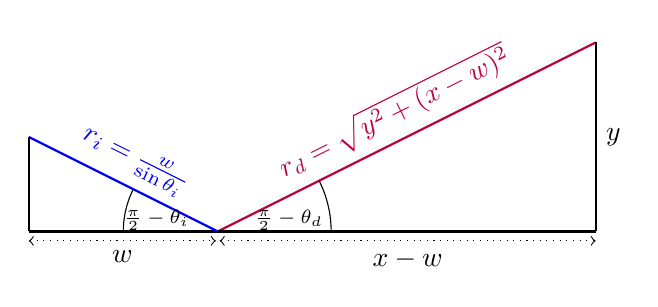
\begin{tikzpicture}[scale=1.2]
                \def\labelOffset{0.1}
                \draw[thick](0,0) -- (2,0);
                \draw[<->,dotted](0,-\labelOffset) -- (2-0.02,-\labelOffset) node[pos=0.5,
                    below]{$w$};
                \draw[thick](0,0) -- (0,1);
                \tikzmath{
                    \firstDiagonalAngle = atan(1/2);
                    \xDiagonalFirst = \labelOffset * sin( \firstDiagonalAngle );
                    \xDiagonalSecond = 2 + \xDiagonalFirst;
                    \yDiagonalFirst = 1 + \labelOffset * cos( \firstDiagonalAngle );
                    \yDiagonalSecond = -1 + \yDiagonalFirst;
                }
                \draw[thick, color=blue](0,1) -- (2,0) node[pos=0.5, above,
                    rotate=-\firstDiagonalAngle]{$r_i= \frac{w}{\sin \theta_i}$};
                %\draw node[pos=0.5, above, rotate=-\firstDiagonalAngle]{$r_i$};
                \def\xArc{1}
                \draw (\xArc,0) arc (180:180-\firstDiagonalAngle:2-\xArc);
                \draw node[] at (\xArc+0.35,0.12)
                    {\begingroup \scriptsize $\frac{\pi}{2} - \theta_i$ \endgroup};
                \tikzmath{
                    \secondDiagonalAngle = atan(2/(6-2));
                }
                \draw[thick, color=purple] (2,0) -- (6,2) node[pos=0.5, above,
                    rotate=\secondDiagonalAngle] {$r_d = \sqrt{y^{2} + (x - w)^{2}}$};
                \draw[thick] (2,0) -- (6,0);
                \draw[thick] (6,2) -- (6,0) node[pos=0.5, right] {$y$};
                \draw[<->,dotted](2+0.02,-\labelOffset) -- (6,-\labelOffset) node[pos=0.5,
                    below]{$x-w$};
                \def\xArc{3.2}
                \draw (\xArc,0) arc (180:180+\secondDiagonalAngle:2-\xArc);
                \draw node[] at (\xArc-0.45,0.12)
                    {\begingroup \scriptsize $\frac{\pi}{2} - \theta_d$ \endgroup};
            \end{tikzpicture}
            \caption{Geometry setup implies that $\frac{1}{r_i r_d} =
                \frac{\sin \theta_i}{ w \sqrt{y^{2} + ( x - w)^{2}} }$, and $\cos \theta_d
                = \frac{y}{\sqrt{y^{2} + ( x - w)^{2}} }$ }
            \label{fig:trigPEC}
            \end{center}
            \end{figure}
            %}}}
%}}}
\newpage
%}}}
% Bibliography {{{
\begin{thebibliography}{1}
   \bibliographystyle{IEEEtran}

   \bibitem{ref:degliSecond}
   V. Degli-Esposti ``A diffuse scattering model for urban propagation prediction'', IEEE Transactions on Antennas and Propagation, vol. 49, no. 7, pp. 1111-1113, July 2001.

   \bibitem{ref:degliThird}
   V. Degli-Esposti, F. Fuschini, E. M. Vitucci and G. Falciasecca, ``Measurement and Modelling of Scattering From Buildings'', IEEE Transactions on Antennas and Propagation, vol. 55, no. 1, pp. 143-153, Jan. 2007.

   \bibitem{ref:directiveRepl}
   F. Mani and C. Oestges, ``Ray-tracing evaluation of diffuse scattering in an outdoor scenario'', Proceedings of the 5th European Conference on Antennas and Propagation (EUCAP), Rome, Italy, 2011.

   \bibitem{ref:BK1}
   Hossein Ragheb, Edwin R. Hancock, ``The modified Beckmann–Kirchhoff scattering theory for rough surface analysis'', Pattern Recognition, Volume 40, Issue 7, 2007, Pages 2004-2020, ISSN 0031-3203.

   \bibitem{ref:BK2}
   F. Sheikh, D. Lessy and T. Kaiser, ``A Novel Ray-Tracing Algorithm for Non-Specular Diffuse Scattered Rays at Terahertz Frequencies'', 2018 First International Workshop on Mobile Terahertz Systems (IWMTS), Duisburg, Germany, 2018, pp. 1-6.

   \bibitem{ref:BK3}
   F. Sheikh and T. Kaiser, ``A Modified Beckmann-Kirchhoff Scattering Model for Slightly Rough Surfaces at Terahertz Frequencies'', 2019 IEEE International Symposium on Antennas and Propagation and USNC-URSI Radio Science Meeting, Atlanta, GA, USA, 2019, pp. 2079-2080.

   \bibitem{ref:reciprocalHeur}
   E. M. Vitucci, N. Cenni, F. Fuschini and V. Degli-Esposti, ``A Reciprocal Heuristic Model for Diffuse Scattering From Walls and Surfaces'', IEEE Transactions on Antennas and Propagation, vol. 71, no. 7, pp. 6072-6083, July 2023.

   \bibitem{ref:fieldPrediction}
   V. Degli-Esposti, D. Guiducci, A. de'Marsi, P. Azzi and F. Fuschini, ``An advanced field prediction model including diffuse scattering'', IEEE Transactions on Antennas and Propagation, vol. 52, no. 7, pp. 1717-1728, July 2004.

   \bibitem{ref:RTComparison}
   M. Zhu, L. Cazzella, F. Linsalata, M. Magarini, M. Matteucci and U. Spagnolini, ``Toward Real-Time Digital Twins of EM Environments: Computational Benchmark for Ray Launching Software'', in IEEE Open Journal of the Communications Society, vol. 5, pp. 6291-6302, 2024.

   \bibitem{ref:dynamicRTPaper}
   Bilibashi, Denis \& Vitucci, Enrico \& Degli-Esposti, Vittorio, ``On Dynamic Ray Tracing and Anticipative Channel Prediction for Dynamic Environments''. IEEE Transactions on Antennas and Propagation. PP. 1-1. 10.1109/TAP.2023.3262155, 2023.

\end{thebibliography}

\end{document}
%}}}
